\begin{frame}[shrink]{Երկկողմանի գրաֆների միջակայքային ներկումներ}
\begin{theorem}[Հանսեն, 1992] Եթե $G$-ն երկկողմանի գրաֆ է, որի համար 
$\Delta(G)\leq 3$, ապա $G\in \mathfrak{N}$ և $w(G)\leq 4$.
\end{theorem}

\begin{itemize}
\item Երկկողմանի գրաֆների միջակայքային ներկումները ուսումնասիրել են Սեվաստյանովը (1991), Գիառոն (1997), Կուբալը, Մալաֆիյսկին (1999) և այլոք:
\end{itemize}

% \begin{theorem}[Գիառո, 1997] Եթե $G$-ն երկկողմանի գրաֆ է, 
% $\Delta(G)=4$ և այն չունի $3$ աստիճան ունեցող գագաթ, ապա $G\in
% \mathfrak{N}$ և $w(G)=4$.
% \end{theorem}

% \begin{theorem}[Գիառո, 1997] $G$ երկկողմանի գրաֆի համար միջակայքային $\Delta(G)$-ներկման գոյությունը կարելի է պարզել բազմանդամային ժամանակում, երբ $\Delta(G)\leq 4$, և $NP$-լրիվ է, եթե $\Delta(G)\geq 5$:
% \end{theorem}

% \begin{theorem}[Գիառո, Կուբալ, Մալաֆիյսկի, 1999] Եթե $G$-ն երկկողմանի գրաֆ է $(X,Y)$ կողմերով, իսկ $\min \{\vert X\vert, \vert Y\vert\}\leq 3$, ապա $G\in
% \mathfrak{N}$:
% \end{theorem}
\end{frame}

\begin{frame}{Միջակայքային ներկում չունեցող երկկողմանի գրաֆներ}
\begin{itemize}
\item Միրումյան, 1989
\item Մալաֆիյսկի, 1999
\item $\Delta(G)=15$, $|V(G)| = 19$
\end{itemize}
\begin{figure}[h]
\begin{center}
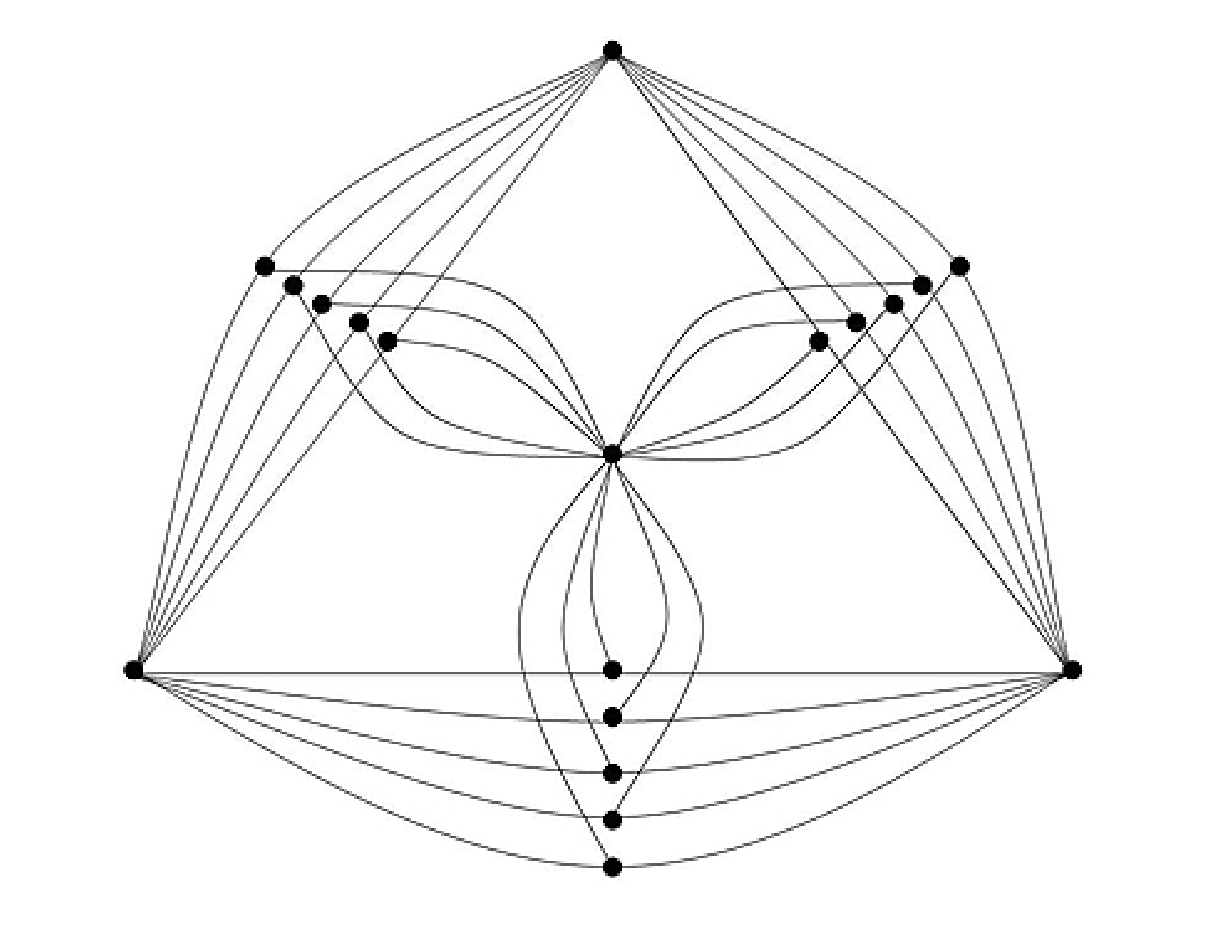
\includegraphics[width=0.6\textwidth]{figures/shannon555.eps}
\end{center}
\end{figure}
\end{frame}


\begin{frame}{Միջակայքային ներկում չունեցող երկկողմանի գրաֆներ}
\begin{itemize}
\item Սեվաստյանով, 1990
\item $\Delta(G)=21$
\end{itemize}

\begin{figure}[h]
\begin{center}
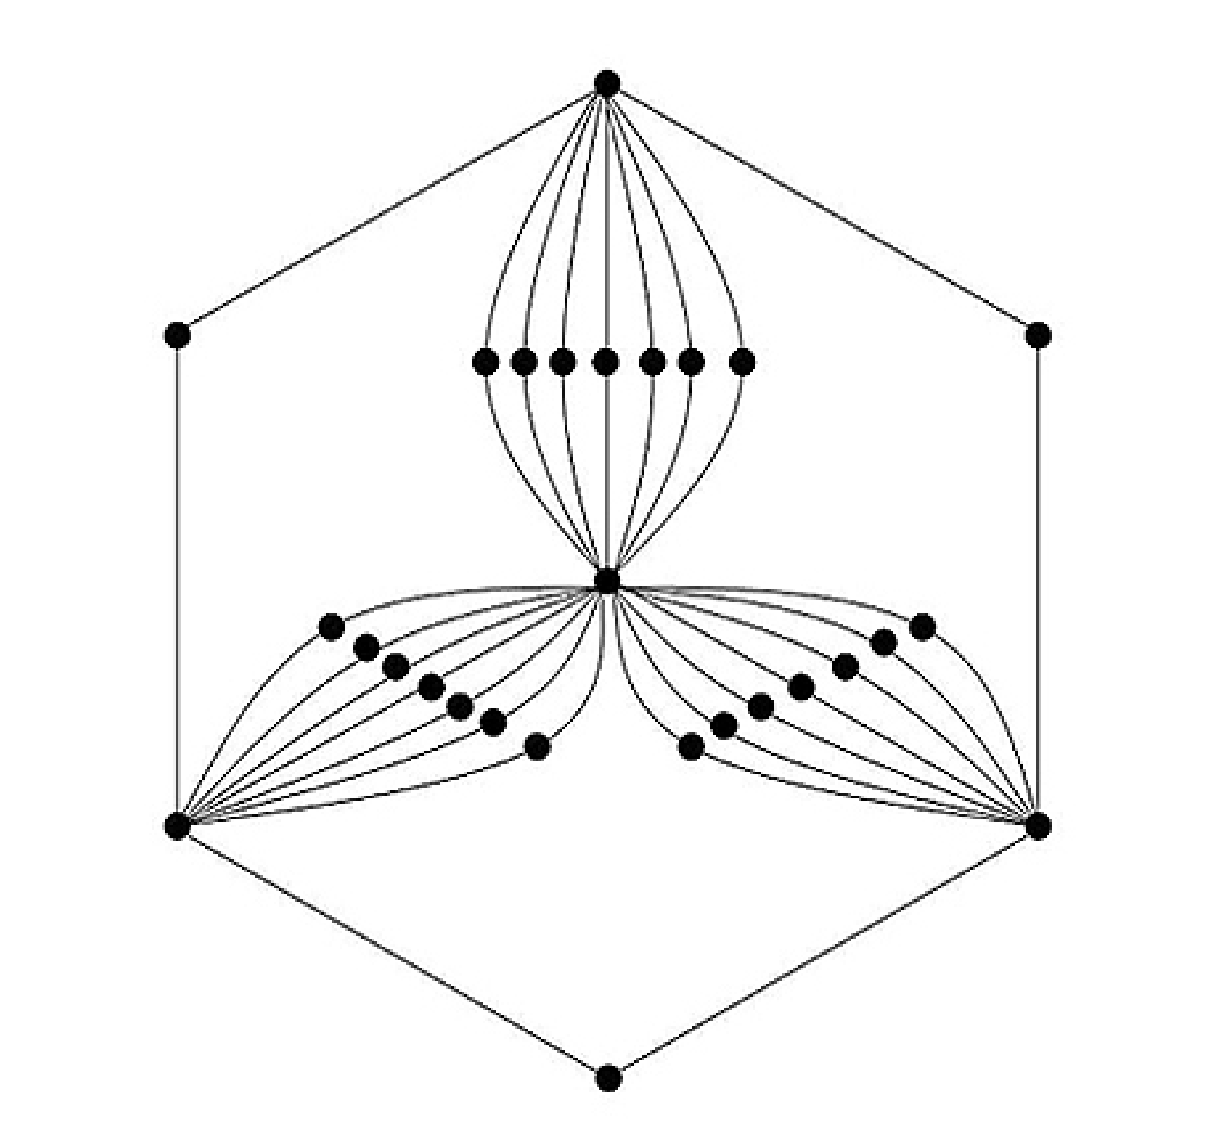
\includegraphics[width=0.6\textwidth]{figures/sevastyanov.eps}
\end{center}
\end{figure}
\end{frame}


\begin{frame}{Միջակայքային ներկում չունեցող երկկողմանի գրաֆներ}
\begin{itemize}
\item Էրդյոշ, 1991
\item $\Delta(G)=13$
\end{itemize}

\begin{figure}[h]
\begin{center}
\includegraphics[width=0.6\textwidth]{figures/erd13.jpg}
\end{center}
\end{figure}
\end{frame}

\begin{frame}[shrink]{Միջակայքային ներկում չունեցող երկկողմանի գրաֆներ}

Ջենսենը և Տոֆտը Graph Coloring Problems (1995) գրքում առաջարկել են հետևյալ խնդիրը.
\begin{problem}
Գոյություն ունի՞ $G$ երկկողմանի գրաֆ, որի համար 
\begin{center}
$4\leq \Delta(G)\leq 12$ և
$G\notin \mathfrak{N}$:
\end{center}
\end{problem}

\pause

Աշխատանքում կառուցվել են միջակայքային ներկում չունեցող երկկողմանի գրաֆների չորս ընտանիքներ.
\begin{enumerate}
    \item Շեննոնի գրաֆների միջոցով կառուցվող հակաօրինակներ
    \item Վերջավոր պրոյեկտիվ երկրաչափություններով հակաօրինակներ
    \item Ծառերի միջոցով կառուցվող հակաօրինակներ
    \item Գրաֆների ենթատրոհումներով կառուցվող հակաօրինակներ
\end{enumerate}
\end{frame}

\begin{frame}{Գրաֆների ենթատրոհումներ}
\begin{itemize}
\item $G$ գրաֆի $S(G)$ ենթատրոհումը ստացվում է $G$-ից՝ յուրաքանչյուր կող մեկ անգամ տրոհելով:
\end{itemize}

\begin{theorem}[Կոստոչկա, 1995; Քամալյան, Միրումյան, 1997; Հանսոն, Լոտեն, Տոֆտ, 1998]
Եթե $G$-ն համասեռ գրաֆ է, ապա $S(G)\in \mathfrak{N}$: 
\end{theorem}
\begin{remark}[3.3.13]
Եթե $G$-ն երկկողմանի գրաֆ է և $G \in \mathfrak{N}$, ապա $S(G)\in \mathfrak{N}$: 
\end{remark}
\pause
\begin{hypothesis}[Պետրոսյան, Խաչատրյան, 2011]
Եթե $G\in \mathfrak{N}$, ապա $S(G)\in \mathfrak{N}$:
\end{hypothesis}

Այս հիպոթեզը հաստատվել է Պյատկինի կողմից (2015):
\end{frame}

\begin{frame}{Գրաֆների ենթատրոհումներով կառուցվող հակաօրինակներ}
\begin{itemize}
\item $G$ գրաֆի $S(G)$ ենթատրոհումը ստացվում է $G$-ից՝ յուրաքանչյուր կող մեկ անգամ տրոհելով:
\item $\widehat{G}$ գրաֆը ստացվում է $S(G)$-ից՝ միացնելով տրոհումից առաջացած գագաթները մի նոր գագաթի:
\end{itemize}
\begin{theorem}[3.3.14]
Եթե $G$-ն կապացված գրաֆ է, և
\begin{center}
$\vert E(G)\vert
> 1+ {\max\limits_{P\in \mathbf{P}}}{\sum\limits_{v\in
V(P)}}\ \left(d_{\widehat{G}}(v)-1\right)$,
\end{center}
որտեղ $\mathbf{P}$-ն $S(G)$-ում տրոհումից առաջացած գագաթները միացնող ամենակարճ շղթաների բազմությունն է, ապա $\widehat{G}\notin \mathfrak{N}$:
\end{theorem}


\end{frame}

\begin{frame}{Միջակայքային ներկում չունեցող երկկողմանի գրաֆներ}
\begin{itemize}
	\item $\Delta(\widehat{K}_{3,4})=12$, $|V(\widehat{K}_{3,4})|=20$
\end{itemize}

\begin{figure}[h]
\begin{center}
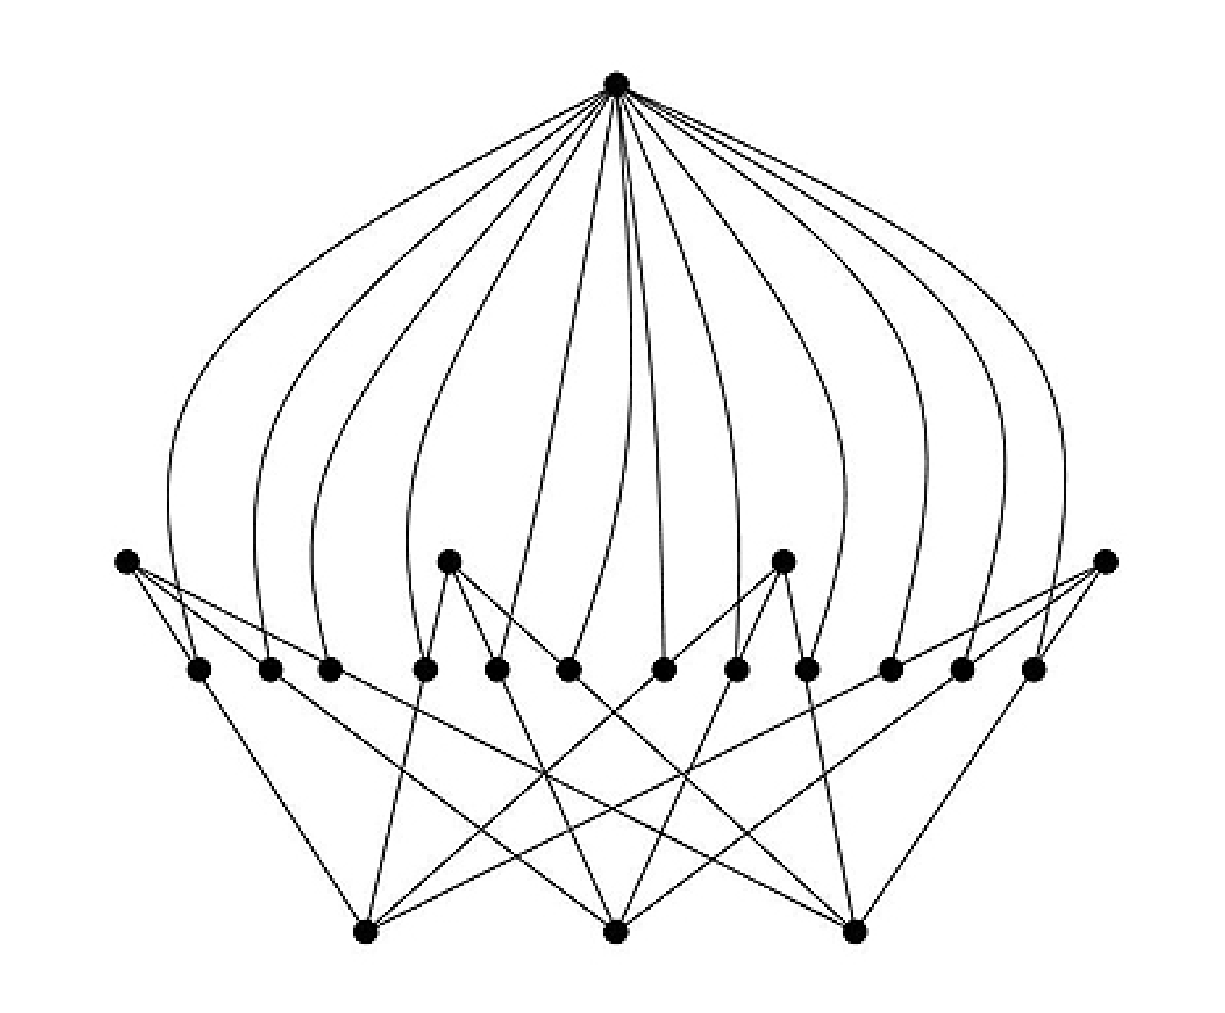
\includegraphics[width=0.5\textwidth]{figures/subdivisionK34.eps}
\end{center}
\end{figure}
\end{frame}


\begin{frame}{Միջակայքային ներկում չունեցող երկկողմանի գրաֆներ}
\begin{itemize}
	\item $\Delta(\widehat{K}_{2,2,2})=12$, $|V(\widehat{K}_{2,2,2})|=19$
\end{itemize}

\begin{figure}[h]
\begin{center}
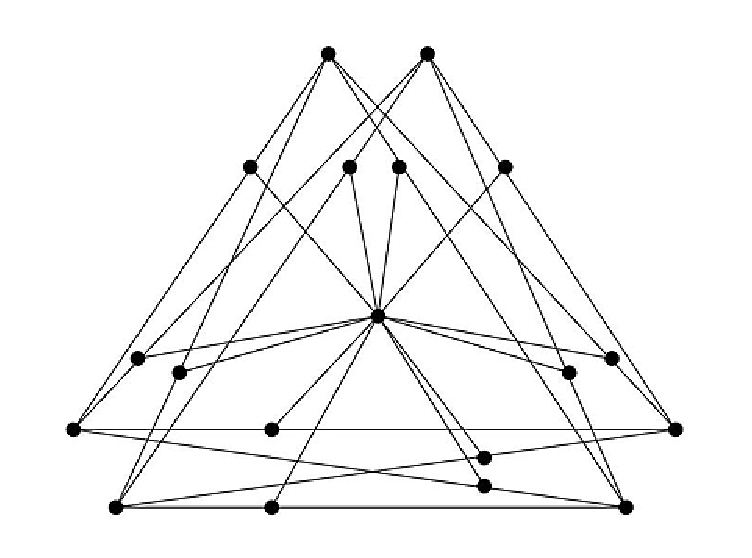
\includegraphics[width=0.5\textwidth]{figures/K222.eps}
\end{center}
\end{figure}
\end{frame}

\begin{frame}{Միջակայքային ներկում չունեցող երկկողմանի գրաֆներ}
\begin{itemize}
	\item $\Delta(\widehat{K}_{3,4}^{\prime})=11$, $|V(\widehat{K}_{3,4}^{\prime})|=20$
\end{itemize}

\begin{figure}[h]
\begin{center}
\includegraphics[width=0.5\textwidth]{figures/K34-prime.jpg}
\end{center}
\end{figure}
\end{frame}


